\section{Manual \& Datasheet}
\arrayrulecolor{gray!45}

\subsection{Board}
\begin{figure}[h]
    \begin{center} 
        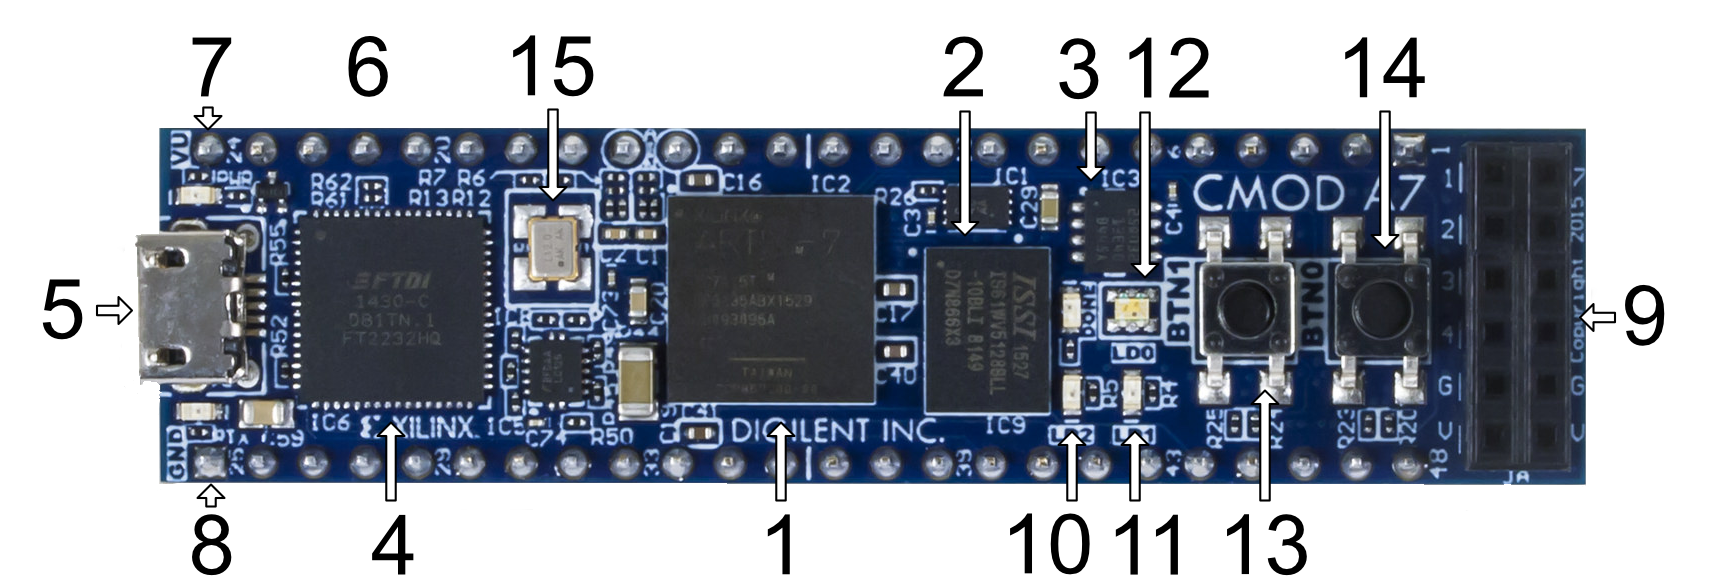
\includegraphics{assets/cmod a7.png}
    \end{center}
    \caption{CMOD A7 Board Description \cite{cmod-a7-topdown}}
\end{figure}
\begin{tabular}{l|l}
    Nr & Description \\ \hline
    1 & Artix-7 FPGA \\
    2 & 512 kB SRAM (only 256 kB usable) \\
    3 & 4 MB FLash (in use for FPGA configuration) \\
    4 & USB-UART Driver \\
    5 & Micro USB Connector \\
    6 & 46 GPIO Pins \\
    7 & 3.3V \\
    8 & GND \\
    9 & PMOD Connector \\
    10 & LED \\
    11 & Status LED \\
    12 & RGB LED \\
    13 & Button \\
    14 & Reset Button \\
    15 & 12 MHz Quartz Oscillator \\
\end{tabular}   

\subsubsection{MCU Status}~\\
The Status LED is on, when the MCU is halted (in boot mode) and can be programmed. \\
Pressing the reset button while the MCU is running restarts the program. \\
Holding the reset button for 2 seconds will bring the MCU into boot mode.\\
When the program ends, the MCU goes into boot mode.
\newpage


\subsection{FPGA Block Diagram}
\begin{footnotesize}Section inspired by \cite{atmega328p-cpu-core} \end{footnotesize}

\begin{figure}[h]
    \begin{center}
        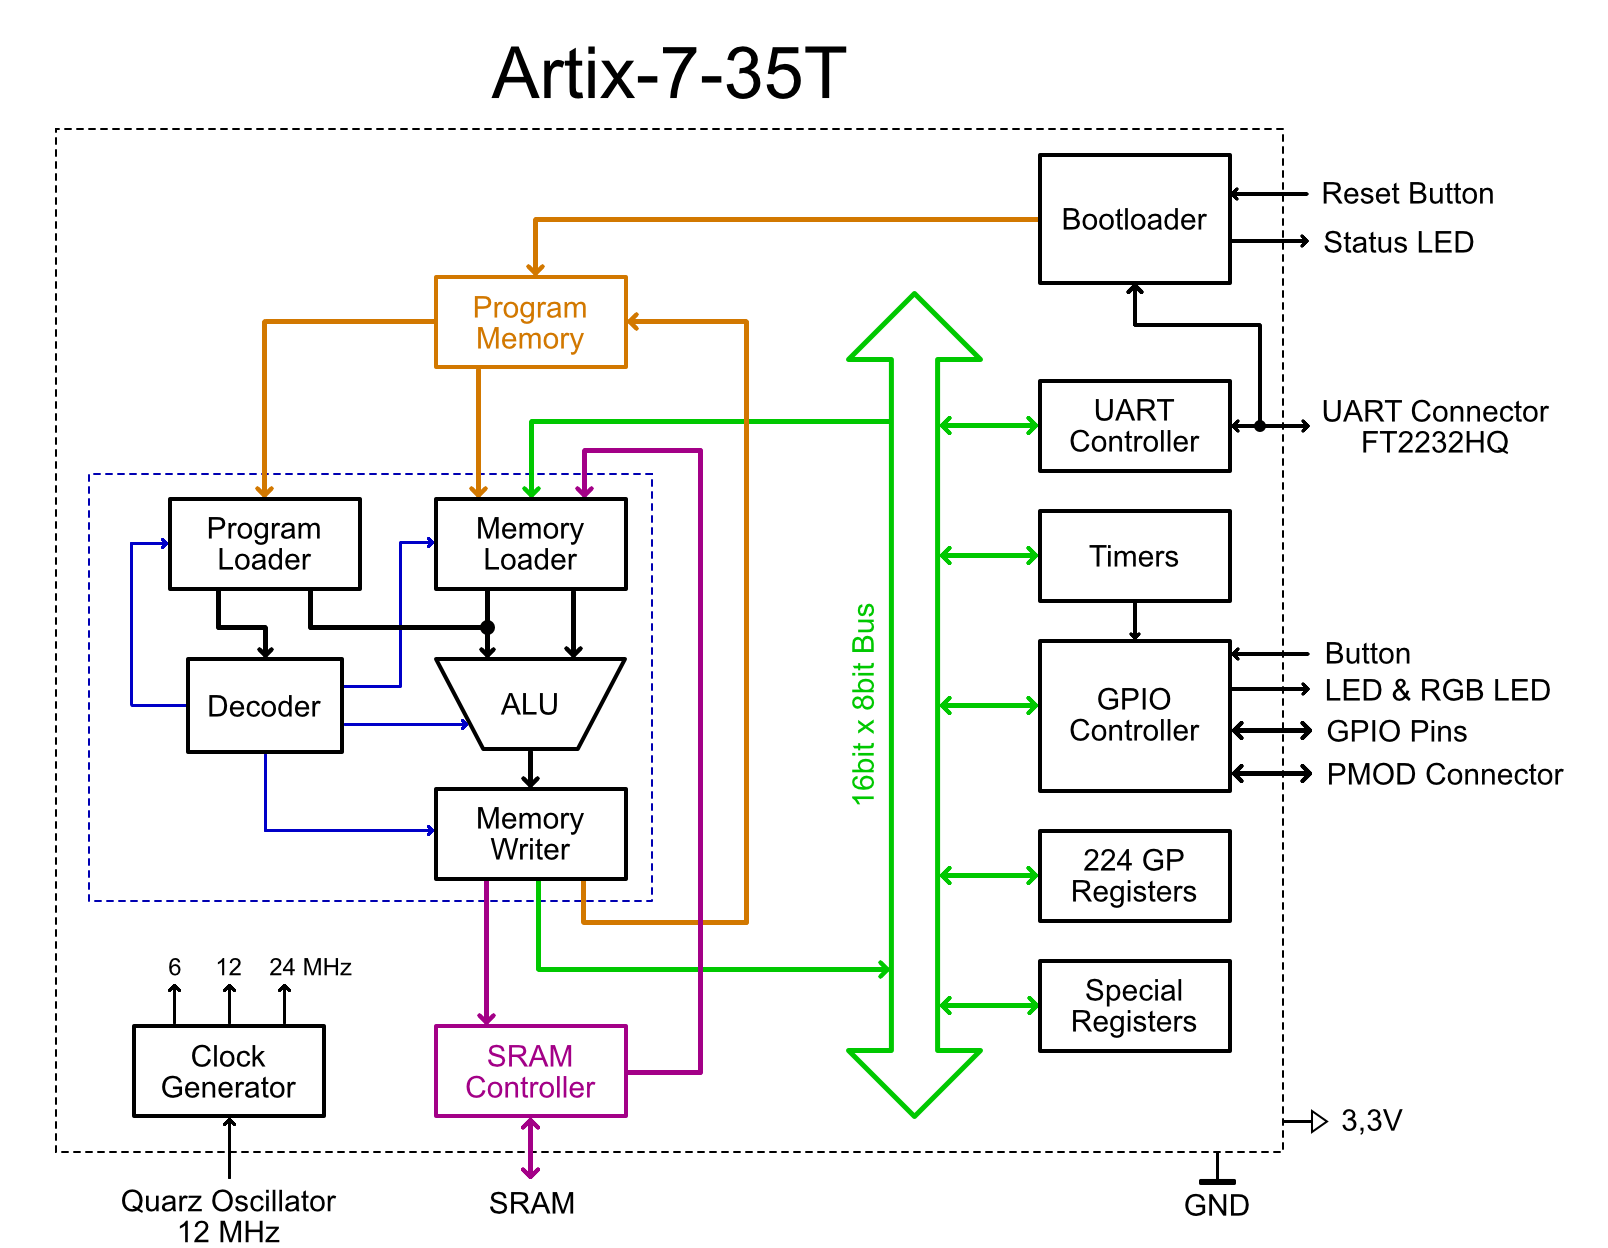
\includegraphics[scale=0.32]{assets/HTMega Blockdesign.png}
    \end{center}
    \caption{FPGA Design Block Diagram}
\end{figure}

The HTMega can be categorized into 2 main parts: 
\begin{itemize}
    \item the central processing unit
    \item the memory, split into: 
    \begin{itemize}
        \item a 8bit address, 16bit data general purpose bus 
        \item a 200 kB internal block memory
        \item a 256 kB external SRAM 
    \end{itemize}
\end{itemize}
Additionally, 6, 12 and 24 MHz internal clock lines are synthesized with a\\ MMCM analog oscillator circuit.\\
A Bootloader circuit is used to write to Program Memory when the MCU is in boot mode.
\newpage

\subsection{Memory}
\begin{footnotesize}Section inspired by \cite{atmega328p-memory} \end{footnotesize}
\subsubsection{General Purpose Bus}
The GP Bus is used to access special internal registers, 224 general purpose registers and peripherals such as UART, Timers and GPIO Pins.\\
Most instructions use these registers as input and/or output. (E.g. ADD, AND, CP, MOV, LDI)\\
There are currently 2 unused addresses at 0xE0 and 0xE1.\\
A list of register addresses and symbols can be found in Section \ref{section:register-symbols} - \nameref{section:register-symbols}.

\subsubsection{Program Memory}
The program memory is a 100k x 16bit Block Memory. One instruction has 32 bit, resulting in memory space for 50 000 instructions.\\
Block RAM is volatile, thus the HTMega has to be reprogrammed once power is lost.\\

The Program Memory can be accessed in program with instructions such as LPM and SPM.\\
The Program Counter addresses 32bit at once, thus the program counter can access the address range of 100k.
To access the whole address range in instructions, 17 bits are needed. The 17th bit is represented by the P flag.

\subsubsection{SRAM}
The CMOD A7 board has a Macronix MX25L3233F 512kB SRAM on board,\\ 256 kB of which are usable.\\
To address the 128k x 16bit, a 17th address bit is needed, represented by the R flag.\\

The SRAM is accessed with instructions such as LD and STM.\\

Instructions such as PUSH and POP use the Stack Pointer register as SRAM address\\
and increment or decrement the Stack Pointer. \newpage


\subsection{Execution Cycle}
Execution happens at a 6 MHz clock cycle and the execution length depends on the instruction.\\
Execution follows this general cycle, depending on the instruction omitting certain operations:
\begin{center}\begin{mdframed}[backgroundcolor=light-gray, roundcorner=10pt,leftmargin=1, rightmargin=1, innerleftmargin=13, innertopmargin=15,innerbottommargin=15, outerlinewidth=1, linecolor=light-gray]
load instruction - decode instruction - load from memory - arithmetic operation - write to memory
\end{mdframed} \end{center}
\paragraph{Example}~\\
\begin{figure}[h]
    \begin{center}
        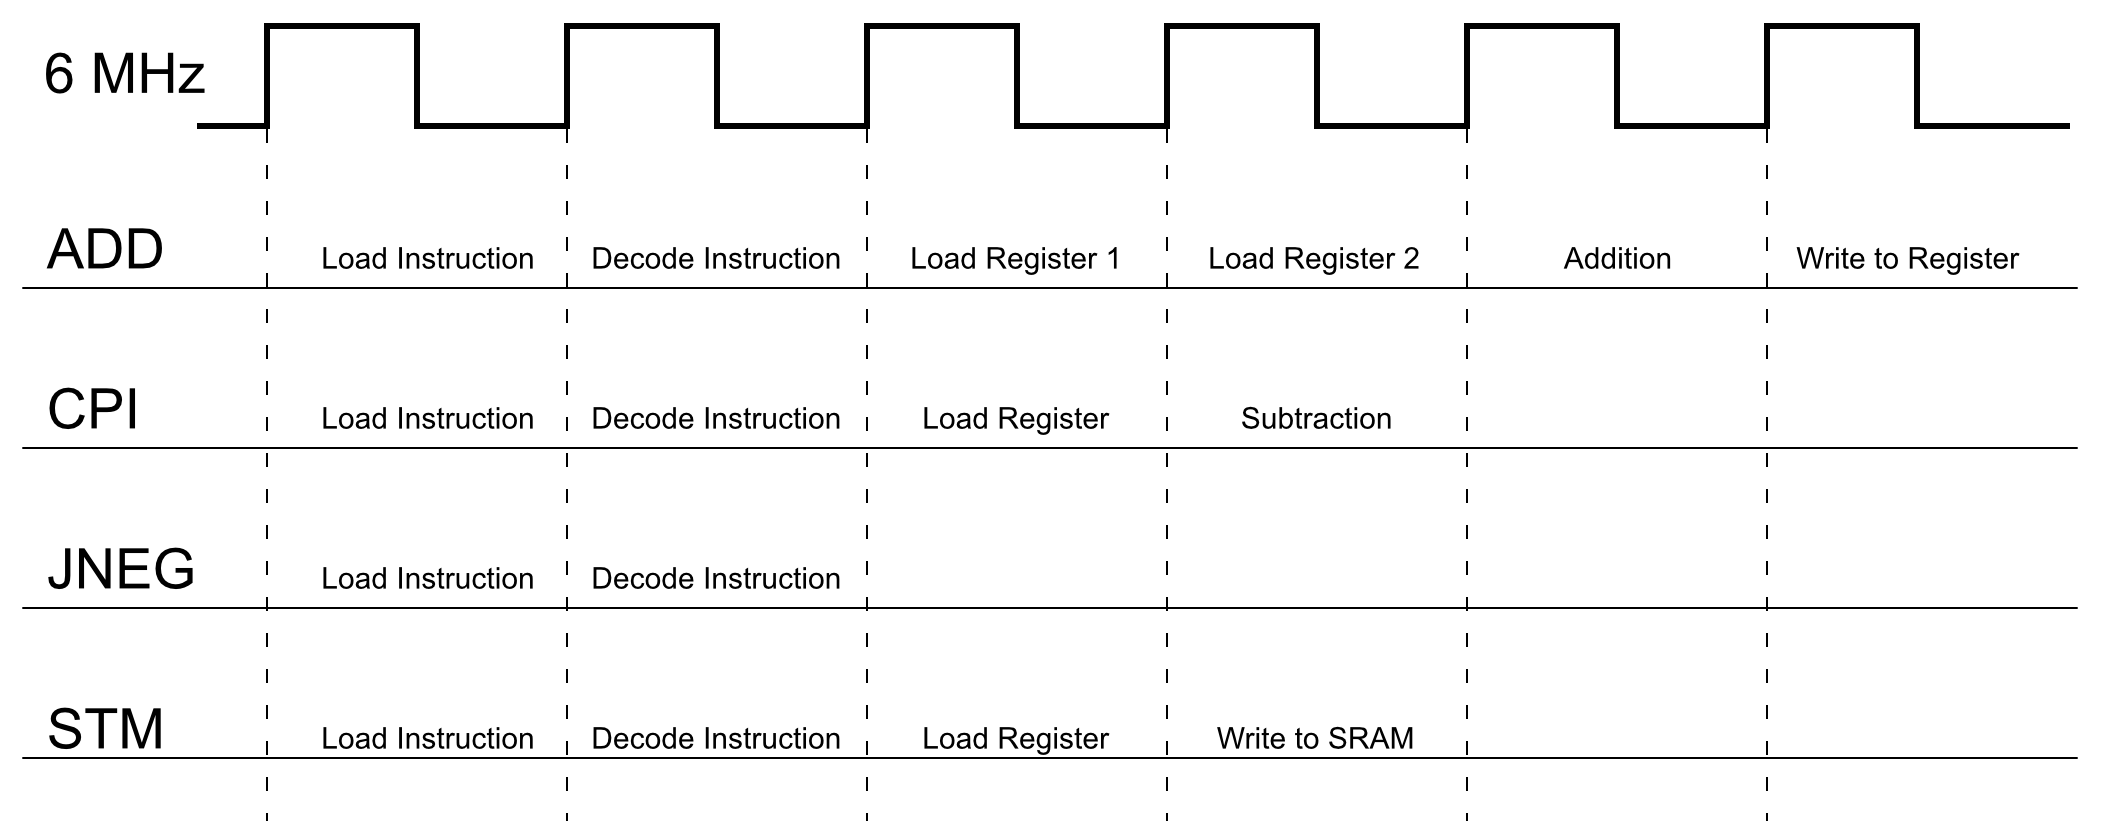
\includegraphics[scale=0.22]{assets/Execution Cycle.png}
    \end{center}
    \caption{Example Execution Cycle}
\end{figure}
\subsection{Programming the Microcontroller}
The program is saved on an internal RAM and thus volatile.\\ Once disconnected, the HTMega will have to be reprogrammed.

\subsubsection{Assembly}
Assembly code consists of consecutive instructions. \\
All instructions for the HTMega can be found in Section \ref{section:instruction-set} - \nameref{section:instruction-set} \\

Every instruction uses 4 bytes of program memory. \\
Labels are yet to be supported, thus you will have to set any jump addresses yourself. Since every instruction has the same length, jump to the instruction line number - 1 (zero-based numbering). \\

Every program ends with an END instruction, if it is missing, the assembler will add it automatically. \\
Any instruction after END will be ignored. \\

Special and IO registers can additionally be addressed with symbols.\\
A list of all Symbols can be found in Section \ref{section:register-symbols} - \nameref{section:register-symbols}.\\
Literal numbers are formatted as binary with 0b and hexadecimal with 0x.\\
Inline comments start with //.\\ ~\\

\paragraph{Example Code}
\begin{mdframed}[backgroundcolor=light-gray, roundcorner=10pt,leftmargin=1, rightmargin=1, innerleftmargin=15, innertopmargin=6,innerbottommargin=6, outerlinewidth=1, linecolor=light-gray]
\begin{lstlisting}[style=hasm]
PUSH PC 0b1011 // push Program Counter to sram address 0b1011 
JMP 0x00 // jump to instruction 0 
END
\end{lstlisting}
\end{mdframed}
An extension for HTMega assembly code highlighting is available for Visual Studio Code and can be installed through a .VSIX file included with the binaries.

\paragraph{Assembling} ~\\
To assemble the script, pass the path of the script to the HTMega assembler:
\begin{mdframed}[backgroundcolor=light-gray, roundcorner=10pt,leftmargin=1, rightmargin=1, innerleftmargin=15, innertopmargin=6,innerbottommargin=6, outerlinewidth=1, linecolor=light-gray]
\begin{lstlisting}[style=hasm]
> HTMegaAssembler.exe <input.hasm> <output.hex>
\end{lstlisting}
\end{mdframed}
Accepted file types are .hasm and .asm for input, .hex and .bin for output.
Omitting the output path will create a output hex file at the same path with the same name as the input.

\subsubsection{Programmer}
To program the HTMega, (re)connect the board over USB or hold the reset button to halt the program.
Then pass the .hex file created by the assembler to HTMegaProgrammer.exe:
\begin{mdframed}[backgroundcolor=light-gray, roundcorner=10pt,leftmargin=1, rightmargin=1, innerleftmargin=15, innertopmargin=6,innerbottommargin=6, outerlinewidth=1, linecolor=light-gray]
\begin{lstlisting}[style=hasm]
> HTMegaProgrammer.exe <input.hex> <COM-Port>
\end{lstlisting}
\end{mdframed}
If no COM-Port is specified, a list of available COM-Ports will be shown to select from.\\

If the COM-Port exists, is not occupied and the HTMega is in boot mode, the assembled binary code is sent to the HTMega and execution is started automatically.

\paragraph{Programming Protocol} ~\\
When the MCU is in boot mode, the Bootloader is listening for the start-byte 0xF0, 
followed by the assembled instructions. The transmission ends with 6x 0xFF.
\newpage


\subsection{Pinout} \label{section:pinout}
\begin{figure}[h]
    \begin{center}
        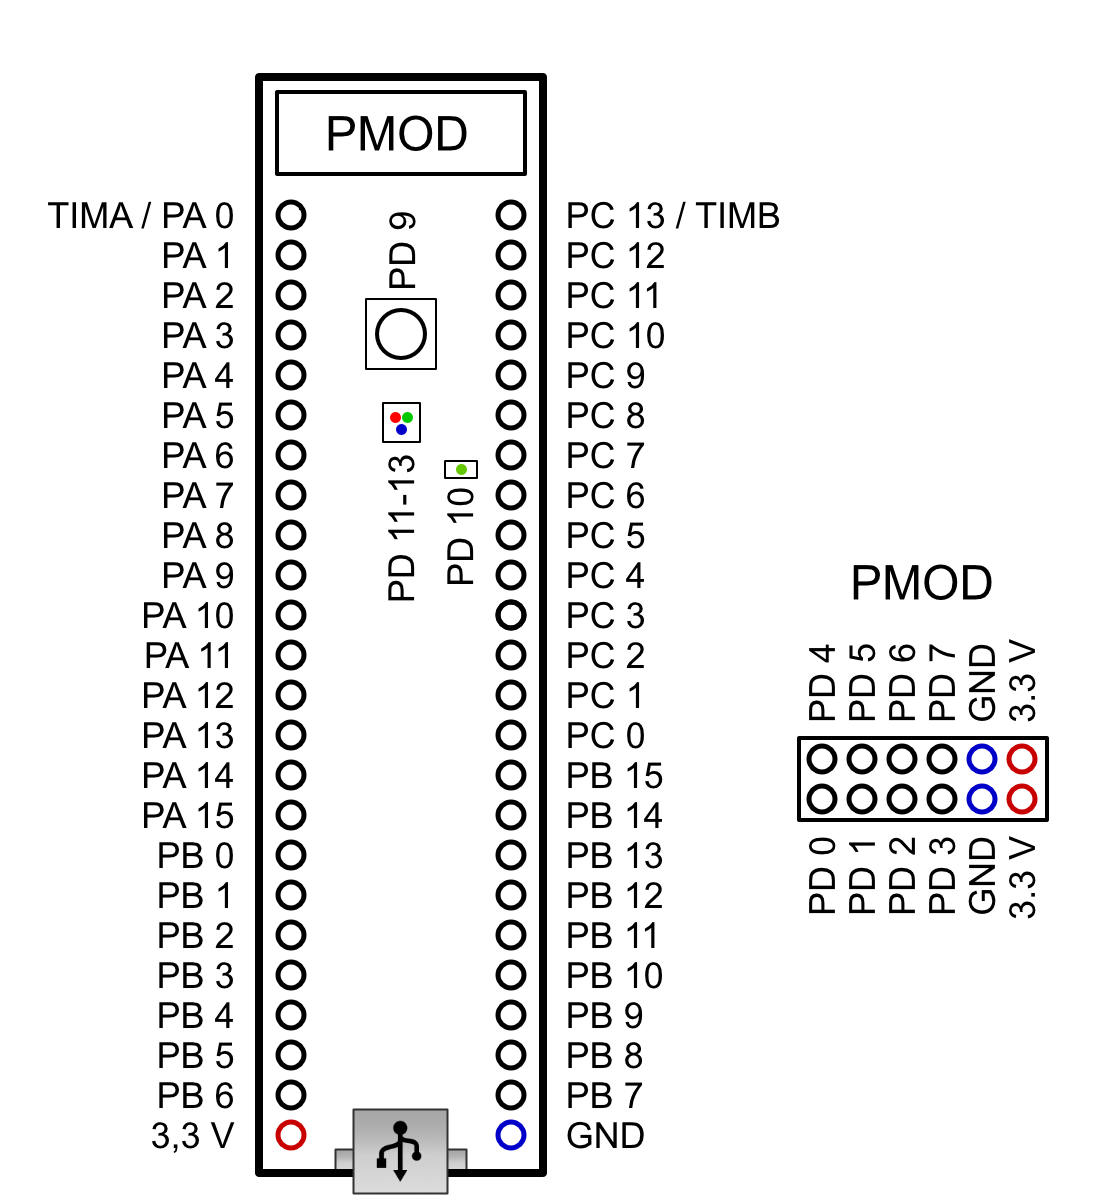
\includegraphics[scale=0.23]{assets/pinout.png}
    \end{center}
    \caption{Pinout \cite{cmod-a7-pinout}}
\end{figure}

\subsection{GPIO} 
\begin{footnotesize}Section inspired by \cite{atmega328p-gpio} \end{footnotesize}\\
As seen in the pinout above, the pins and IOs are split into 4 register groups.\\
Port A-C control the breadboardable pins, Port D controls onboard IO like LEDs and buttons,\\
as well as the PMOD connector.\\

All pins are digital and can take the states 3.3V or 0V, matching 1 or 0 in the registers.\\
Each group consists of three registers: input, output and output enable. (Px\_in, Px\_out, Px\_conf)\\

The input register matches the state the pins have. The output register sets the state of a pin.\\ 
All GPIO pins and PMOD pins are set to high impedance by default,\\ so when connecting a voltage from the outside, there won't be a short circuit.\\
To connect a bit in the output register to the assigned pin, the associated bit in the output enable register has to be 1.\\

The onboard LED (PD 10) and RGB LED (PD 11 = red, PD 12 = green, PD 13 = blue) are always connected to the output register. Output enable has no effect on these pins.\\
The onboard button (PD 9) is never connected to the output register.
When output enable is set to 0 for pins PA 0 and PC 13, they are connected to Timer A and Timer B. 
\newpage


\paragraph{Block Diagram}~\\
\begin{figure}[h]
    \begin{center}
        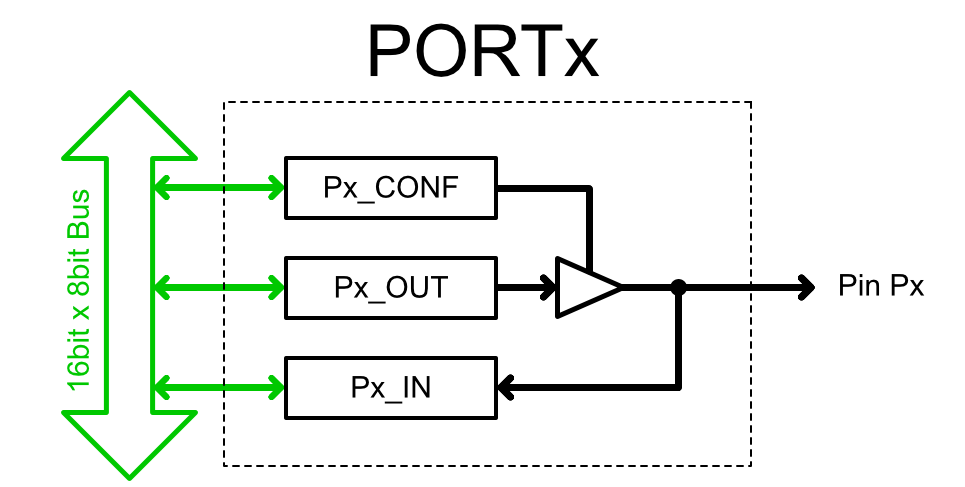
\includegraphics[scale=0.3]{assets/GPIO.png}
    \end{center}
    \caption{GPIO Interface Block Diagram}
\end{figure}
\paragraph{Example Code}
\begin{mdframed}[backgroundcolor=light-gray, roundcorner=10pt,leftmargin=1, rightmargin=1, innerleftmargin=15, innertopmargin=6,innerbottommargin=6, outerlinewidth=1, linecolor=light-gray]
\begin{lstlisting}[style=hasm]
LDI pa_conf 0b100   // enable PA 2 output
LDI pa_out 0b100    // set PA 2 to 1
XORI pd_out 0x200   // toggle onboard LED 
END
\end{lstlisting}
\end{mdframed}


\subsection{USB - UART}
The CMOD A7 board has a FT2232HQ USB-UART converter enabling UART communication over UART for the HTMega.

\subsubsection{Protocol}
UART protocol as found in \cite{uart}
A UART frame used by the HTMega consists of: 1 low start bit, 8 data bits, an even or odd parity bit, 2 high stop bits.
The max baud rate is 6 MHz and can be reduced by the baud rate divider.\\
12 bits with a maximum baud rate of 6 MHz results to a maximum data transfer rate of 500 kB/s 
\begin{figure}[h]
    \begin{center}
        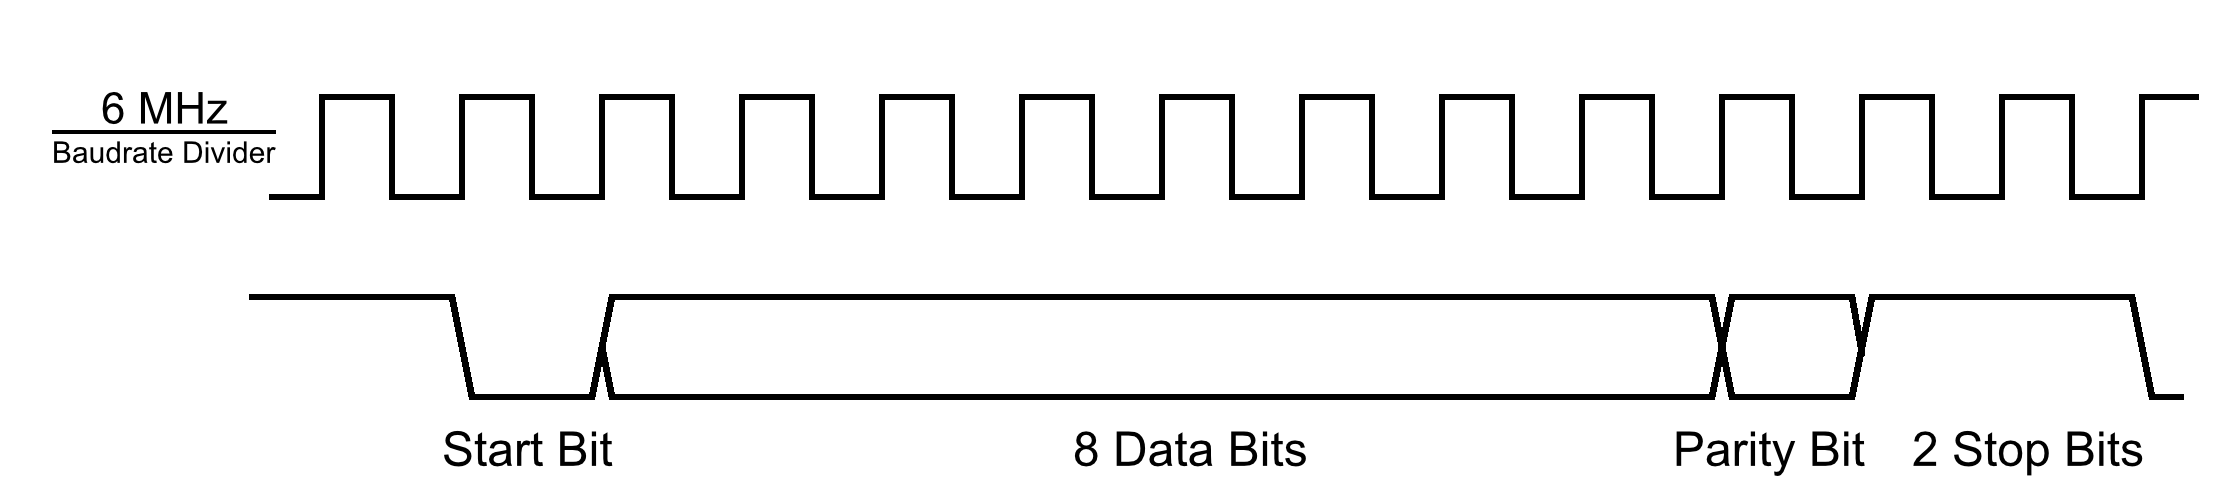
\includegraphics[scale=0.2]{assets/UART.png}
    \end{center} 
    \caption{UART Frame}
\end{figure}
\newpage


\subsubsection{Configuration}
UART configuration is stored in the register UART\_CONF.\\

\begin{tabular}{|P{120mm}|P{15mm}|P{15mm}|}
    \rowcolor{gray!50}
    \hline
    15 - 2 & 1 & 0\\
    \hline
    Baud Rate Divider & Parity & Enable \\
    \hline
\end{tabular}\\~\\

\begin{tabular}{@{}p{35mm}|p{60mm}}
    Enable & Enable Sending and Receiving\\
    Parity & Even parity (0), Odd parity (1)\\ 
    Baud Rate Divider & Set UART Baud rate
\end{tabular}

\begin{flalign} 
    & UART\; Baud\; Rate = \frac{6 MHz}{Baud\; Rate\; Divider} &
\end{flalign}\\
If the Baud Rate Divider is 0, the Baud rate is set to 6 MHz.

\subsubsection{Sending}
Transmission data is stored in the Register UART\_TD. Enable has to set to 1 to enable transmission.\\
Writing to UART\_TD starts the transmission and the lower byte of UART\_TD will be transmitted.
While the transmission is active, the 'sending' bit in UART\_RD is 1.

\subsubsection{Receiving}
UART status and received data are stored UART\_RD.\\
Once enabled, the UART controller is always listening for UART frames coming over USB.\\
While a frame is being received, 'receiving' in UART\_RD is 1.\\
Once the frame is fully received, 'received' is set to 1 and the received data is 
transferred to 'Received Data' in UART\_RD. If the parity of the received frame does not match the set parity 
(even by default), 'wrong parity' is set to 1.

\paragraph{UART\_RD Register Description}~\\

\begin{tabular}{|P{25mm}|P{22mm}|P{16mm}|P{15mm}|P{14mm}|P{45mm}|}
    \rowcolor{gray!50}
    \hline
    15 - 12 & 11 & 10 & 9 & 8 & 7 - 0\\
    \hline
    x & wrong parity & received & receiving & sending & Received Data\\
    \hline
\end{tabular}\\~\\

\begin{tabular}{@{}p{26mm}|p{100mm}}
    Received Data & Data of the last received UART frame\\
    sending & Status: is currently sending\\ 
    receiving & Status: is currently receiving\\
    received & Status: finished receiving current UART frame\\
    wrong parity & Status: wrong parity in the last received UART frame\\
\end{tabular}\\

Writing to UART\_RD won't overwrite any data, but will reset 'wrong parity', 'received' and 'Received Data'.
\newpage

\subsection{Timers}
\begin{footnotesize}Section inspired by \cite{atmega328p-timers} \end{footnotesize}\\
The HTMega has 2 universal 16 bit timers/counters and a 32 bit microseconds counter.

\subsubsection{Universal Timer/Counter}
The Universal 16bit Timer/Counter is a binary counter with a configurable top value,\\
a comparison unit and the ability to generate PWM on a certain pin.\\
For the actual position of the IO pin, refer to section \ref{section:pinout} - \nameref{section:pinout}.

\begin{figure}[h]
    \begin{center}
        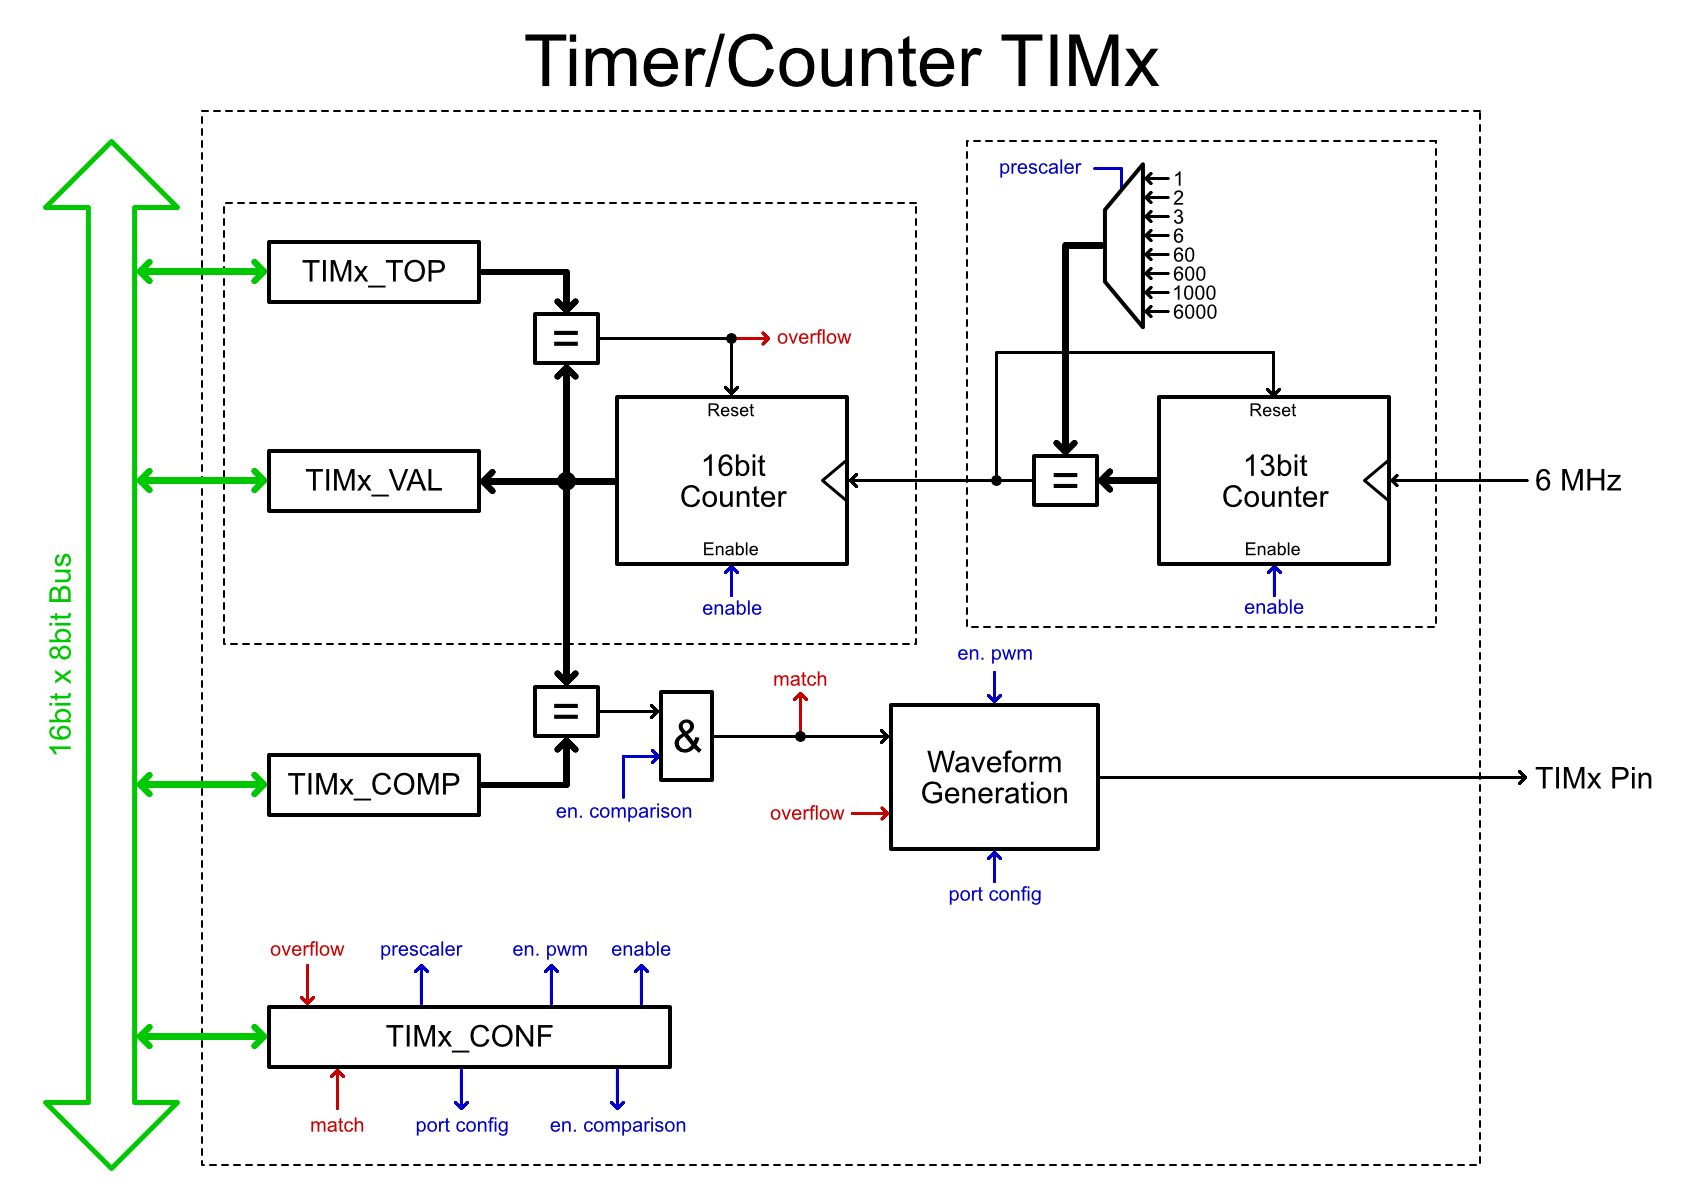
\includegraphics[scale=0.28]{assets/TIMx.png}
    \end{center}
    \caption{Universal Timer/Counter Block Diagram}
\end{figure}
\newpage 


\subsubsection{Configuration}
Timer/Counter configuration and status are stored in TIMx\_CONF.\\

\begin{tabular}{|P{18mm}|P{14mm}|P{15mm}|P{18mm}|P{20mm}|P{15mm}|P{18mm}|P{14mm}|}
    \rowcolor{gray!50}
    \hline
    15 - 10 & 9 & 8 & 7 - 5 & 4 - 3 & 2 & 1 & 0 \\
    \hline
    x & match & overflow & prescaler & port config & en. pwm & en. comp. & enable\\
    \hline
\end{tabular}\\ ~\\

\begin{tabular}{@{}p{22mm}|p{100mm}}
    match & Status: counter value matched comparison value\\
    overflow & Status: counter reached top\\ 
    Prescaler & select prescaler value \\
    Port Config & configure waveform generation \\
    en. pwm & enable waveform generation \\
    en. comp & enable comparison \\
    enable & enable Timer/Counter 
\end{tabular}

\paragraph{Prescaler}~\\
The prescaler reduces the counter input clock frequency.\\ A prescaler value can be selected from a preset of 8 values.\\

{ % section with table coloring
\rowcolors{2}{gray!25}{white}
\begin{tabular}{|p{20mm}|p{14mm}|p{14mm}|p{14mm}|p{14mm}|p{14mm}|p{14mm}|p{14mm}|p{14mm}|}
    \rowcolor{gray!50}
    \hline
    Prescaler & 000 & 001 & 010 & 011 & 100 & 101 & 110 & 111 \\
    \hline
    Divider & 1 & 2 & 3 & 6 & 60 & 600 & 1000 & 6000 \\
    \hline
    Frequency & 6 MHz & 3 MHz & 2 MHz & 1 MHz & 100 kHz & 10 kHz & 5 kHz & 1 kHz\\
    \hline
\end{tabular}~\\

\paragraph{Waveform Generation}~\\
Port Config configures the behaviour of the assigned port.\\

en. pwm = 0\\
\begin{tabular}{|p{20mm}|p{100mm}|}
    \rowcolor{gray!50}
    \hline
    Port Config & Operation\\\hline
    00 & none \\ \hline
    01 & toggle port on match \\ \hline
    10 & reset port on match \\ \hline
    11 & set port on match \\ \hline
\end{tabular}\\

en. pwm = 1\\
\begin{tabular}{|p{20mm}|p{100mm}|}
    \rowcolor{gray!50}
    \hline
    Port Config & Operation\\\hline
    00 & none \\ \hline
    01 & toggle port on match \\ \hline
    10 & fast PWM: set port on zero, reset port on match \\ \hline
    11 & reverse PWM: reset port on zero, set port on match\\ \hline
\end{tabular}
}